%% LyX 1.4.1 created this file.  For more info, see http://www.lyx.org/.
%% Do not edit unless you really know what you are doing.
\documentclass[11pt,a4paper,english,masters,answers]{article}
\usepackage[latin1]{inputenc}
\setcounter{secnumdepth}{3}
\setcounter{tocdepth}{3}
\usepackage{graphicx}

\makeatletter

%%%%%%%%%%%%%%%%%%%%%%%%%%%%%% LyX specific LaTeX commands.
%% Bold symbol macro for standard LaTeX users
\providecommand{\boldsymbol}[1]{\mbox{\boldmath $#1$}}

%% Because html converters don't know tabularnewline
\providecommand{\tabularnewline}{\\}

%%%%%%%%%%%%%%%%%%%%%%%%%%%%%% Textclass specific LaTeX commands.
 \usepackage{pslatex}
 \usepackage{myexam}
 \usepackage{graphicx}
 \usepackage{amsmath}
 \usepackage{epic}
 \usepackage{eepic}
 \input{neilutils}
\newenvironment{lyxcode}
{\begin{list}{}{
\setlength{\rightmargin}{\leftmargin}
\setlength{\listparindent}{0pt}% needed for AMS classes
\raggedright
\setlength{\itemsep}{0pt}
\setlength{\parsep}{0pt}
\normalfont\ttfamily}%
 \item[]}
{\end{list}}

%%%%%%%%%%%%%%%%%%%%%%%%%%%%%% User specified LaTeX commands.
\newcommand{\answer}[2]{}
\newcommand{\masters}[2]{#2}

\usepackage{babel}
\makeatother
\begin{document}

\pressmark{\masters{COM6131}{COM3270}}


\examtitle{NETWORK PERFORMANCE ANALYSIS}


\examdate{AUTUMN SEMESTER 2004--2005}


\examtime{2 HOURS}

\begin{exam}
~

\turnover

\masters{\center{\Large\textbf{Section A}\normalsize}}{}

\begin{question}
This question concerns queueing models based around birth-death processes,
\emph{i.e.} Markov arrivals and Markov departures.
\begin{qupart}
Explain what you understand by the term utilization factor. What are
the advantages and disadvantages of utilisation factors that are close
to one? 

\mypercent{25}

\end{qupart}
\answer{

The utilization factor is a measure of the \emph{efficiency of the
system}. It is the \emph{percentage of time} that the servers are
in use. A high utilization factor means that a \emph{high proportion
of the available resources are being used} which is an \emph{}advantage.
The \emph{}disadvantage \emph{i}s that for utilization factors which
are close to one the queue occupancy is likely to be very high and
\emph{queueing delays} will be large resulting in poor quality of
service. \textbf{\emph{Five for each italicised statement.}} }{0}

\begin{qupart}
Give the utilization factors for the following queues: $M/M/1$, $M/M/1/m$,
$M/M/m$ and $M/M/\infty$. 

\mypercent{20}

\answer{

\begin{center}\begin{tabular}{|c|c|c|}
\hline 
Queue&
\multicolumn{2}{c|}{Conditions}\tabularnewline
\hline
\hline 
$M/M/1$&
$\rho=\frac{\lambda}{\mu}$&
\begin{tabular}{c}
Where $\mu$is the service rate \tabularnewline
\hline 
and $\lambda$ is the arrival rate.\tabularnewline
\hline
\end{tabular}\tabularnewline
\hline 
$M/M/1/m$&
$\rho=\left(1-P\left(m\right)\right)\frac{\lambda}{\mu}$&
\begin{tabular}{c}
Where $\mu$is the service rate, $\lambda$ is the arrival rate\tabularnewline
\hline 
and $P\left(m\right)$ is the blocking probability.\tabularnewline
\hline
\end{tabular} \tabularnewline
\hline 
$M/M/m/m$&
$\rho=\frac{\lambda}{m\mu}$&
\begin{tabular}{c}
Where $\mu$is the service rate, $\lambda$ is the arrival rate and\tabularnewline
$m$ is the number of servers.\tabularnewline
\end{tabular} \tabularnewline
\hline 
$M/M/\infty$&
$\rho$doesn't really exist&
\begin{tabular}{c}
The value doesn't exist because there are infinite servers\tabularnewline
\hline 
the probability that any part of the system is in use is $1-P\left(0\right)=1-\exp\left(-a\right)$\tabularnewline
\hline
\end{tabular} \tabularnewline
\hline
\end{tabular}\par\end{center}

\textbf{\emph{Five for each queue}}}{0}

\end{qupart}
~

\begin{qupart}
What do you understand by the term `blocking probability'? Give the
blocking probability for the $M/M/m/m$ and $M/M/1/m$ queues.

\mypercent{20}

\end{qupart}
\answer{In queues with finite size (such as $M/M/1/m$) customers
that arrive when the queue is full are blocked. The probability of
this happening in steady state is known as the blocking probability.

\begin{center}\begin{tabular}{|c|c|c|}
\hline 
Queue&
\multicolumn{1}{c|}{Blocking probability}&
\tabularnewline
\hline
\hline 
$M/M/1/m$&
$P\left(m\right)=\frac{\rho^{m}\left(1-\rho\right)}{1-\rho^{m+1}}$&
Where $\rho=\frac{\lambda}{\mu}$ is the utilisation factor.\tabularnewline
\hline 
$M/M/m/m$&
$B(m,a)=P\left(m\right)=\frac{\frac{a^{m}}{m!}}{\sum_{n=0}^{m}\frac{a^{n}}{n!}}$ &
Where $a=\frac{\lambda}{\mu}$ is the offered load.\tabularnewline
\hline
\end{tabular}\par\end{center}

\textbf{\emph{Ten for statement, five for each blocking probability.}}}{0}

\begin{qupart}
Describe what you understand by the \emph{steady state distribution}
of a queueing system.

\mypercent{15}

\end{qupart}
\answer{The steady state distribution of a queue is the distribution
\emph{stationary distribution} that the Markov chain converges to.
It occurs when a \emph{dynamic equilibrium} is obtained in the queueing
system. A dynamic equilibrium is when change in one direction is balanced
(on average) by change in the opposite direction. The steady state
distribution is \emph{used for making predictions} about the expected
states of the queue.

\textbf{\emph{Five for each italicised statement.}}}{0}

\begin{qupart}
For the $M/M/1$, $M/M/m$, $M/M/m/m$ and the $M/M/\infty$ queues
give the conditions under which the steady state distribution will
exist.

\mypercent{20}

\end{qupart}
\answer{The steady state condition exists for each of these queues
when the following conditions are satisfied:

\begin{center}\begin{tabular}{|c|c|c|}
\hline 
Queue&
\multicolumn{2}{c|}{Conditions}\tabularnewline
\hline
\hline 
$M/M/1$&
$\lambda<\mu$&
The arrival rate is lower than the service rate.\tabularnewline
\hline 
$M/M/m$&
$\lambda<m\mu$&
The arrival rate is lower than $m$ times the service rate.\tabularnewline
\hline 
$M/M/1/m$&
No conditions&
The steady state distribution always exists.\tabularnewline
\hline 
$M/M/\infty$&
No conditions&
The steady state distribution always exists.\tabularnewline
\hline
\end{tabular}\par\end{center}

\textbf{\emph{Five marks for each queue.}}}{0}

\end{question}
\continued

\masters{\center{\Large\textbf{Section B}\normalsize}}{}

\begin{question}
The diagram below gives the state diagram for a discrete time $M/M/1$
queue.

\begin{center}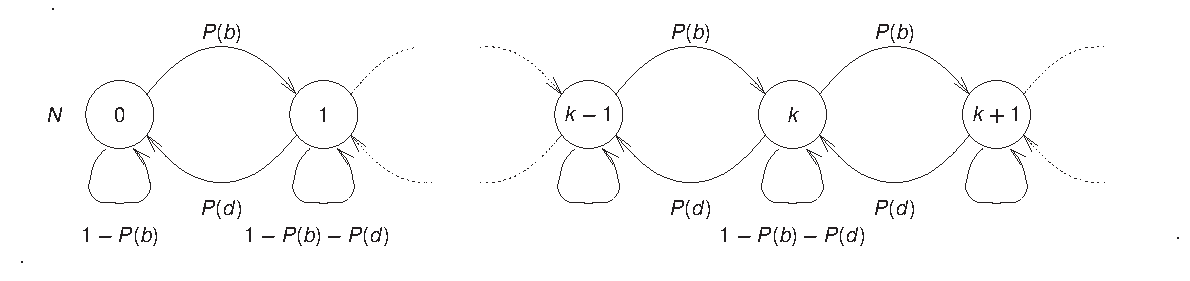
\includegraphics[width=1\textwidth]{diagrams/discreteMM1State}\par\end{center}

In the system you may take the probability of a birth to be $P\left(b\right)=\lambda\delta t$
and the probability of a death to be $P\left(d\right)=\mu\delta t$,
where $\delta t$ is the change in time for each time step and $\left(\mu+\lambda\right)\delta t<1$.

\begin{qupart}
Derive the steady state distribution for this queue in terms of its
utilization factor.\label{qup:steadyState}

\mypercent{30}

\end{qupart}
~\answer{As a birth-death process the stationary distribution of
the queue may be found using detailed balance. We therefore look at
the flow across a boundary between two states.

\begin{center}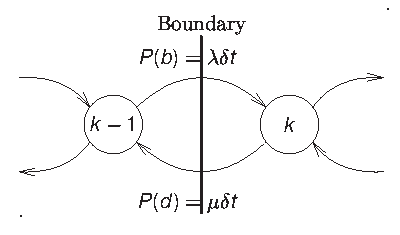
\includegraphics{diagrams/boundaryFlowDiscreteMM1}\par\end{center}

For this flow to balance we must have, at steady state,\[
P\left(k\right)P\left(d\right)=P\left(k-1\right)P\left(b\right)\]
\[
P\left(k\right)\mu\delta t=P\left(k-1\right)\lambda\delta t\]
\[
P\left(k\right)\mu=P\left(k-1\right)\lambda\]
\[
P\left(k\right)=\frac{\lambda}{\mu}P\left(k-1\right)\]
Taking the utilisation factor $\rho=\frac{\lambda}{\mu}$ we have
\[
P\left(k\right)=\rho P\left(k-1\right)\]
\[
P\left(k\right)=\rho^{k}P\left(0\right)\]
Using the normalisation condition to find $P\left(0\right)$ \[
\sum_{k=0}^{\infty}P\left(k\right)=1\]
\[
P\left(0\right)\sum_{k=0}^{\infty}\rho^{k}=1\]
The infinite series converges for $\rho<1$ (equivalent to $\mu>\lambda$)
giving\[
\sum_{k=0}^{\infty}=\frac{1}{1-\rho}\]
 substituting back in we have\[
P\left(0\right)=1-\rho\]
and finally\[
P\left(k\right)=\rho^{k}\left(1-\rho\right)\]
which is recognised as a geometric distribution.

\textbf{\emph{5 for the boundary flow diagram 10 for the correct value
in terms of $P\left(0\right)$, 10 for the correct derivation of $P\left(0\right)$
and 5 for the right answer.}}}{0}

\begin{qupart}
Derive the mean of this distribution.

\mypercent{20}

\end{qupart}
~\answer{The mean has the form \[
\left\langle k\right\rangle =\sum_{k=0}^{\infty}k\rho^{k}\left(1-\rho\right)\]
Extracting one $\rho\left(1-\rho\right)$ we have \[
\left\langle k\right\rangle =\rho\left(1-\rho\right)\sum_{k=0}^{\infty}k\rho^{k-1}\]
which is recognised as\[
\left\langle k\right\rangle =\rho\left(1-\rho\right)\frac{d}{d\rho}\sum_{k=0}^{\infty}\rho^{k}\]
which can be written\[
\left\langle k\right\rangle =\rho\left(1-\rho\right)\frac{d\left(1-\rho\right)^{-1}}{d\rho}\]
\[
\left\langle k\right\rangle =\rho\left(1-\rho\right)\frac{1}{\left(1-\rho\right)^{2}}\]
\[
\left\langle k\right\rangle =\frac{\rho}{1-\rho}.\]
\textbf{\emph{5 for the correct formula for the mean, 10 for the differentiation
trick and 5 for the correct answer.}{0}}}

\begin{qupart}
Write down an algorithm for computer simulation of this queue. You
may use MATLAB notation or pseudocode to express your algorithm.

\mypercent{30}

\end{qupart}
~

\answer{

\begin{lyxcode}
lambda~=~1;~~\%~birth~rate

mu~=~2;~~~\%~death~rate

deltat~=~0.01;~\%~time~step

k~=~0;~~\%~Initial~state~of~queue

T~=~100000;~\%~a~number~of~time~steps

for~i~=~1:T~\\
~~p~=~rand(1);~\%~a~uniform~random~number~between~0~and~1

~~if~p~<~lambda{*}deltat

~~~~k~=~k~+~1;

~~elseif~p~<~(lambda+mu){*}deltat~\&~k~>~0

~~~~k~=~k~-~1;

~~end

end~\\

\end{lyxcode}
\textbf{\emph{10 marks for overall structure of code, 5 for random
number generation 5 for first if statement and 10 for second if statement
(5 for each condition).}{0}}}

\begin{qupart}
When designing networks we are normally interested in the steady state
behaviour of the system. For simple queues such as the discrete time
$M/M/1$ we can compute this analytically. If we cannot compute it
analytically we have to resort to simulation. What problems could
occur with the simulation you described in part c) which might mean
you do not accurately estimate the steady state distribution? You
may wish to base your answer around the three different averages:
distribution, sample based and time.

\mypercent{20}

\end{qupart}
\answer{Typically in queueing problems we are interested in expectations
under steady state distribution. Ideally we want to compute the steady
state distribution's average, which we can do for the discrete $M/M/1$
queue. However for more complex queueing systems we may not be able
to compute this average in which case we try and approximated it with
a sample based average. Typically these approximations involve sampling
from a Markov chain. Averaging these values directly leads to a time
based average, for a sample based average we need to samples to be
\emph{independent}. To estimate the sample based average accurately
we do not take every sample from the Markov chain, but we wait between
samples.

Finally if the effective state space is large (the state space that
the queue is likely to visit) then we may have to wait a long time
for enough samples to get an accurate idea of the steady state distribution,
it is also difficult to tell how long we need to wait.

\textbf{\emph{10 for averages correctly described. 5 for understanding
sample based average vs time dependent and 5 for saying we may not
run simulation long enough.}}}{0}

\end{question}
~

\turnover

\begin{question}
\textbf{Delay analysis of an ARQ System.} In an automatic repeat request
(ARQ) system packets are transmitted in frames that are 1 millisecond
long. An acknowledgement is sent if a packet is received without error.
The system waits for a maximum of $n-1$ milliseconds to receive the
acknowledgement. Once the acknowledgement is received the next packet
in the queue is transmitted. A schematic of this system is shown below.

\begin{center}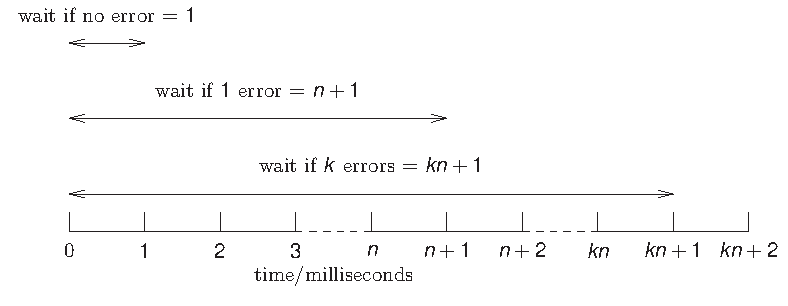
\includegraphics[width=0.8\textwidth]{diagrams/ARQ}\par\end{center}

For the purposes of the analysis below you can take probability of
an error in a packet to be $p$ and you may assume that errors occur
statistically independently. Finally you may assume that arrivals
occur as a Poisson process with a rate $\lambda$.

\begin{qupart}
Explain why the probability distribution for the time interval between
the start of the transmission of a given packet and the end of the
previous transmission (the service time distribution) is given by\[
P\left(X=1+kn\right)=\left(1-p\right)p^{k}\]


\mypercent{15}

\end{qupart}
\answer{The distribution represents the probability that there are
$k$ errors followed $p^{k}$ followed by a successful transmission
$\left(1-p\right)$. The length of time that this takes will be $n$
for each failure (1 for transmission and $n-1$ waiting for the acknowledgement
) plus the length of transmission for a single packet. \textbf{\emph{five
for k retransmission probability 5 for successful transmission probability
and 5 for associated length of time.}} }{0}

\begin{qupart}
What is the mean of this distribution?

\mypercent{25}

\end{qupart}
\answer{\begin{eqnarray*}
\left\langle X\right\rangle  & = & \sum_{k=0}^{\infty}\left(1+kn\right)\left(1-p\right)p^{k}\\
 & = & \left(1-p\right)\left(\sum_{k=0}^{\infty}p^{k}+n\sum_{k=0}^{\infty}kp^{k}\right)\\
 & = & 1+\frac{np}{1-p}\end{eqnarray*}
 \textbf{\emph{May also need to compute the sum of}} kp\textasciicircum{}k.
\textbf{\emph{10 for mean formula, 5 for first line, 10 for result.}}}{0}

\begin{qupart}
What is the utilization factor for this queue?

\mypercent{10}

\end{qupart}
\answer{The utilization is simply the arrival rate multiplied by
the average service time.\[
\rho=\frac{\lambda\left(1-p\right)}{1-p+np}\]
and thus \[
1-\rho=\frac{1-\lambda-p\left(n-1-\lambda\right)}{1-p+np}\]
}{0}

\begin{qupart}
What is the second moment of the service time distribution?

\mypercent{30}

\end{qupart}
\answer{\begin{eqnarray*}
\left\langle X^{2}\right\rangle  & = & \sum_{k=0}^{\infty}\left(1+kn\right)^{2}\left(1-p\right)p^{k}\\
 & = & \left(1-p\right)\left(\sum_{k=0}^{\infty}p^{k}+2n\sum_{k=0}^{\infty}kp^{k}+n^{2}\sum_{k=0}^{\infty}k^{2}p^{k}\right)\\
 & = & 1+\frac{2np}{1-p}+\frac{n^{2}\left(p+p^{2}\right)}{\left(1-p\right)^{2}}\end{eqnarray*}
\textbf{\emph{10 for each line.}}}{0}

\begin{qupart}
Comment on the validity of the independence assumption you have made
for the packet errors.
\end{qupart}

\mypercent{20}

\answer{In practice, this assumption is probably unrealistic. If
an error occurs due to problems in the transmission channel (such
as interference) it is likely that several packets in a row will not
be received, so the errors do not occur independently. Also the assumption
of a fixed probability of packet error may be incorrect, \emph{e.g.}
it may vary with load.}{0}

\textbf{\emph{You may find the following formula useful in your derivations:}}
$\sum_{k=0}^{\infty}k^{2}p^{k}=\frac{p+p^{2}}{\left(1-p\right)^{3}}$.

\end{question}
~

\continued

\begin{question}
When simulating networks of queues we have to resort to approximations.
In this question we will review some of the issues that arise when
performing these approximations.
\begin{qupart}
A small system is modelled as two queues. Packets arrive at the first
queue as a Poisson stream with exponentially distributed packet lengths.
After leaving the first queue the packets enter a second queue. The
service time for each packet at both queues is proportional to each
packet's length. Explain how the second queue's size, as perceived
by an arriving packet, will be related to the arriving packet's length.
How will this affect the waiting time for the arriving packet at the
second queue? 

\mypercent{25}

\end{qupart}
~\answer{The longer packets will arrive at the second queue to find
a shorter queue than the shorter packets. Or in other words queue
length at the second queue are anti correlated with packet lengths.
This is because, while the longer packet was being served at the first
queue there is time for the second queue to empty out. This is analogous
to a slow moving truck driver who will generally see an open road
in front of him.

\textbf{\emph{10 marks for correctly saying that the queue will be
shorter for longer packets (or vice versa). 10 Marks for saying the
longer packet will wait less time at the second queue. 5 marks for
analogy (given in course text and notes).}} }{0}

\begin{qupart}
Explain what you understand by Kleinrock's independence assumption.
Given this assumption, what is the delay for a transmission line with
a traffic rate of $\lambda$ and an average transmission time of $\bar{X}$?

\mypercent{25}

\end{qupart}
~\answer{Kleinrock's independence assumption is an assumption that
a packets service time at a node in a network of queues is statistically
independent of its service time at any other node in the queueing
model. \textbf{\emph{}}In the approximation you assume each communication
link is an $M/M/1$ \textbf{\emph{}}queue. This means the delay is
given by\[
\bar{T}=\frac{1}{\mu_{ij}-\lambda_{ij}}=\frac{\bar{X}}{1-\rho}\]
where $\rho=\lambda\bar{X}$, the utilization factor. \textbf{\emph{10
marks for the first sentence or equivalent meaning.}} \textbf{\emph{15
marks for the approximation of the communication links as an $M/M/1$
queue}} \emph{and correct formula}.}{0}

\begin{qupart}
Give conditions under which Kleinrock's independence assumption will
yield a reasonable approximation for a network of queues.

\mypercent{25}

\end{qupart}
~\answer{Kleinrock suggested that when different traffic streams
are merged to form a single stream the approximation becomes reasonable.
Particularly if that traffic is a large volume from outside the network
and is Poisson distributed. The approximation also is better for single
path routing algorithms. (Example 3.17 in Bertsekas and Gallagher)
\textbf{\emph{10 marks for merging of streams. 10 marks for if the
additional traffic is Poisson and from outside the network. 5 marks
for the single path routing algorithms.}} Note that in practice students
also suggested Medium/Medium-Heavy traffic loads, Poisson arrivals
and exponential service times and densely connected networks, I gave
a maximum of 12 marks for answers which mentioned these issues but
failed to mention any of the above.}{0}

\begin{qupart}
What does Jackson's theorem state and what are its assumptions? What
is the average number of packets in a system according to Jackson's
theorem?

\mypercent{25}

\end{qupart}
~\answer{Jackson's theorem states that if packet interarrival times
after passing through the first queue are not correlated with their
lengths (Kleinrock's independence assumption) and if randomisation
is used to divert traffic along the different routes then the average
number of packets in the system can be derived as if each queue where
$M/M/$1. This gives the number of packets in the system as\[
\bar{N}=\sum_{ij}\frac{\lambda_{ij}}{\lambda_{ij}-\mu_{ij}}\]
where $\lambda_{ij}$ is the traffic flow rate between node $i$ and
$j$ and $\mu_{ij}$ is the average service time between node $i$
and node $j$. \textbf{\emph{10 marks for randomisation and 5 for
Kleinrock. 10 marks for formula.}{0}}}

\end{question}
\questionsend

\end{exam}

\end{document}
